\subsection*{1.1}
%1. Build the circuit shown below using BS170 transistor and a resistor RD = 470 . %Supply
%voltage is VDD = +15 V. Transistor gate is connected to a variable power supply.   
The circuit in figure 1 was built using the NI Elvis experimental setup using a drain resistor, $R_D$ measured as $462 \Omega$.

    %FIG1 CIRCUIT DIAGRAM OF A HALFWAVE RECTIFIER
    \begin{figure}[h!]
        \centering
        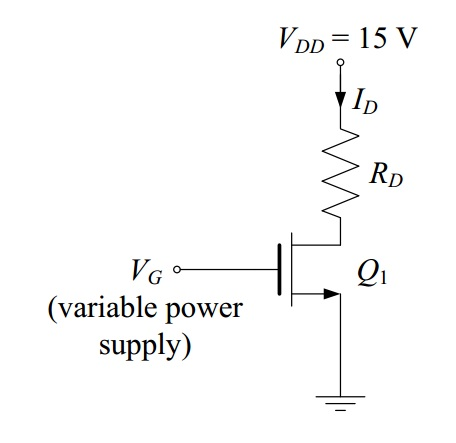
\includegraphics[width=6cm]{circuit_task_1.jpg}
        \captionof{figure}{The circuit in Task 1}
    \end{figure}

\subsection*{1.2}
% 2. Determine the threshold voltage and the transconductance parameter k of the MOS
%transistor. 
%In particular, find the voltage VT for which noticeable drain current appears,
The threshold voltage was determined by observing the drain current while increasing the voltage at the gate. The threshold voltage was determined at the point where an increase of the gate voltage caused a significant change in the drain current. The threshold voltage was determined by doing a polynomial fit to the data collected and an exact value found to be be $V_T = 1.86 \ V$.

   \begin{table}[htbp]
     \centering
     \caption{Data for the gate voltage versus drain current}
       \begin{tabular}{cc}
       $V_{G_0}$ [V]       & $I_{D_0}$ [mA] \\
       0.00         & -1.537 \\
       0.28         & -1.521 \\
       0.56         & -1.523 \\
       0.75         & -1.537 \\
       1.03         & -1.530 \\
       1.31         & -1.532 \\
       1.50         & -1.534 \\
       1.69         & -1.444 \\
       1.80         & -0.608 \\
       1.85         & -0.550 \\
       1.90         & 0.923 \\
       2.00         & 3.950 \\
       2.10         & 9.255 \\
       2.20         & 17.100 \\
       2.30         & 25.700 \\
       2.40         & 32.380 \\
       \end{tabular}%
     \label{tab:addlabel}%
   \end{table}%


The transconductance factor was estimated by taking one point from the graph when $V_G > V_T$. The point chosen was $I_{D_0}  = 9.255 \ mA  \approx 10 \ mA$ and corresponding gate voltage is $V_{G_0} = 2.1 \ V$. Therefore: $$ k = \dfrac{I_{D_0}}{(V_{G_0}-V_T)^2} = \dfrac{9.255 \ mA}{(2.1 \ V - 1.86 \ V)^2} = 160.78 \ \dfrac{mA}{V^2} $$

\begin{figure}[h!]
        \centering
        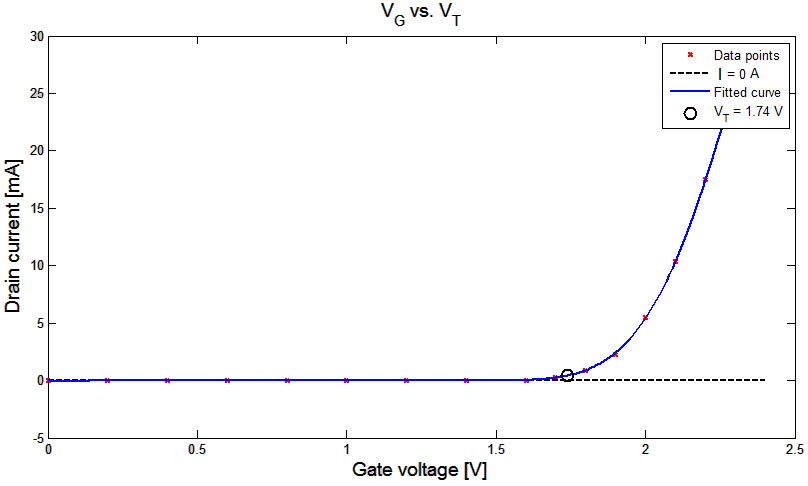
\includegraphics[width=16cm]{Task1_matlab.png}
        \captionof{figure}{Plot of the drain current versus the gate voltage ($I_D$ vs. $V_G$)}
\end{figure}
%This data can also be estimated by measuring the voltage over $R_D$ and then calculating $I_D = \dfrac{V_{DD}-V_D}{R_D}$ as suggested in the assignment. This gives the same results as measuring the current as done here above.

%Note that the parameter k here includes W/L and 0.5 factor
%that you have in the drain current formula ID = 0.5 kn’W/L(VGS–VT)2, i.e., k = 0.5kn’W/L.
\pagebreak